% !TeX program = pdflatex -shell-escape

\documentclass{article}
% \usepackage[T1]{fontenc}
\usepackage[utf8]{inputenc}
\usepackage{amsmath, amssymb,amsfonts}
\usepackage{graphicx}
\usepackage{hyperref}
\usepackage{minted}
\usepackage{setspace}
\usepackage{tikz}
\usetikzlibrary{positioning, shapes.misc, arrows}


\newcommand*{\defeq}{\stackrel{\text{def}}{=}}
\newcommand{\quotes}[1]{``#1''}


\title{MCMC in Text Generation}
\author{Shlok Mishra}
\date{April 2024}

\begin{document}
\doublespacing
\thispagestyle{empty}
\pagenumbering{roman}
% \vspace*{0.5cm}
\begin{center}
    \textbf{ \Large
        Text Generation with MCMC\\
    }
    \vspace*{1cm}
    \textbf{Undergraduate Project}
    \vspace*{1cm}

    By \\
    \vspace*{1cm}
    \textbf{Shlok Mishra}
    \textbf{(210991)}

    \textbf{BS Statistics and Data Science}
    \vspace*{1cm} \\
    Under the guidance of

    \textbf{Prof. Dootika Vats}
    \vspace*{1cm}
    \begin{center}
        
\includegraphics[width=0.25\textwidth]{iitklogo.jpg}
    \end{center}

    \textbf{Department of Mathematics and Statistics, \\ Indian Institute of Technology, Kanpur \\ April, 2024}
\end{center}

\newpage
\onehalfspacing
\thispagestyle{empty}
\vspace*{2cm}
\begin{center}
    \textbf{\underline{Declaration}}
\end{center}
\vspace*{1cm}
{I/We hereby declare that the work presented in the project report entitled "Text Generation with MCMC" contains my own ideas in my own words. At places, where ideas and words are borrowed from other sources, proper references, as applicable, have been cited. To the
    best of our knowledge this work does not emanate from or resemble other work created
    by person(s) other than mentioned herein.}
\vspace*{2cm}

\noindent Date: \hspace{7.5cm} Prof. Dootika Vats


\newpage
\vspace*{3cm}
\section*{Abstract}
In this project, we conduct a thorough examination of the COLD paper, delving into the nuances of its implementation. Our in-depth analysis reveals inaccuracies within their Langevin MCMC implementation, prompting us to explore alternative methodologies. Consequently, we adopt the Barker MCMC approach for sampling, which stands as a methodologically sound alternative. This shift allows us to address the identified shortcomings and implement a framework that leverages the Barker proposal MCMC method for effective solution space exploration. Our focus is on utilizing gradient information to make probabilistic decisions about accepting or rejecting updates, which is crucial for meeting both hard and soft text generation constraints. Our experiments across various text generation tasks, such as lexically-constrained generation, abductive reasoning, and counterfactual reasoning, demonstrate the superior performance of our approach over traditional methods. This project not only rectifies the limitations found in the COLD paper's implementation but also showcases the potential of the gradient-informed Barker MCMC in enhancing the quality of constrained text generation.
\newpage
\tableofcontents





\newpage
\newpage
\pagenumbering{arabic}


\section{Introduction}

In the realm of natural language processing, generating text that is not only linguistically fluent but also adheres to specific semantic or stylistic constraints has emerged as a pivotal challenge. These constraints vary widely, from hard lexical requirements ensuring the inclusion of specific keywords in the output, to soft topical constraints aimed at contextualizing the generated text within a certain narrative or theme. For instance, in knowledge-grounded or keyword-guided text generation tasks, it is crucial to incorporate predetermined keywords as non-negotiable elements of the output. Similarly, tasks may demand the generation of text that logically bridges the past and future contexts of a narrative through abductive reasoning, or modifies an input text to reflect a new, counterfactual condition while maintaining semantic coherence and minimal edits relative to the original text.

Traditionally, tackling these varied requirements has predominantly relied on supervised learning models, trained on datasets meticulously annotated to reflect each unique combination of constraints. However, the dynamism and diversity of constraint combinations pose a significant challenge, rendering the annotation process both impractical and resource-intensive. Furthermore, the advent of large-scale models like GPT-3 has introduced additional complexities, as the feasibility of training such behemoths for specific tasks becomes increasingly untenable. This backdrop underscores a critical need for decoding algorithms that can efficiently leverage pretrained language models, enabling them to navigate complex constraint landscapes without necessitating task-specific fine-tuning.

Our project introduces a novel constrained decoding methodology that conceptualizes the decoding process as a sampling activity from an energy-based model (EBM). By defining an energy function that encapsulates arbitrary constraint functions tailored to the task at hand, our approach facilitates sampling from the distribution induced by the EBM. This project is the first to apply the Barker proposal mechanism, a Markov Chain Monte Carlo (MCMC) method, within the context of text-based EBMs, enabling gradient-informed sampling for discrete text generation. Through iterative updates to a continuous relaxation of the text, guided by the gradients of the energy function, our method—named Constrained Decoding with Barker Dynamics (CDBD)—enables the generation of text sequences that are not only fluent but also in strict adherence to the specified constraints.

In this report, we first delve into the foundational terms and concepts that underpin the natural language processing paradigm, setting the stage for a comprehensive understanding of the field. Following this, we explore the methodology and implementation as presented in the COLD paper, highlighting its contributions to constrained text generation. We then critically analyze the challenges associated with their Langevin MCMC implementation, particularly focusing on the issues arising from the use of adaptive optimizers in a stochastic sampling context. Building on this critique, we introduce our novel Barker MCMC proposal, a methodologically distinct approach designed to overcome these limitations. Our report culminates in a demonstration of the Barker MCMC's superiority, showcasing its robustness and efficiency through empirical testing across a variety of text generation tasks. This journey through the report not only illuminates the evolving landscape of constrained text generation but also underscores our innovative contributions to enhancing the decoding process through the integration of gradient-based dynamics.

\section{Background}

This section lays the groundwork for understanding the pivotal concepts in natural language processing (NLP) that inform our study, particularly focusing on language models, word embeddings, neural text generation, and constrained text generation. These concepts are essential for grasping the complexities of generating text that is not only coherent and contextually relevant but also adheres to specified constraints.

A \textbf{Language Model} (LM) is a pivotal tool in NLP, trained on extensive text corpora to learn linguistic properties such as syntax, semantics, and context implicitly. This foundational understanding enables the model to generate text or perform tasks with human-like language comprehension without explicit rule-based programming.

\textbf{Word Embeddings} provide a sophisticated means to represent words as vectors in a high-dimensional space, encapsulating semantic meanings. This representation allows for the quantitative assessment of word similarity, with closer vectors in the embedding space indicating higher semantic similarity. Formally, given a vocabulary \(V\) and an embedding space \(\mathbb{R}^d\), each word \(w \in V\) is mapped to a vector \(\mathbf{v}_w \in \mathbb{R}^d\), optimizing this mapping based on contextual usage patterns. The similarity between two words \(w_1\) and \(w_2\) is computed as:
\begin{equation}
    \text{similarity}(\mathbf{v}_{w_1}, \mathbf{v}_{w_2}) = \frac{\mathbf{v}_{w_1} \cdot \mathbf{v}_{w_2}}{\|\mathbf{v}_{w_1}\| \|\mathbf{v}_{w_2}\|},
\end{equation}
which facilitates a myriad of applications from clustering to analogy solving.

\textbf{Neural Text Generation} encompasses modeling the distribution of text sequences and employing decoding algorithms for generation. It involves factorizing the sequence probability into per-token conditional probabilities, parameterized by neural networks like transformers. This process is represented by:
\begin{equation}
    p_{\theta} = \prod_{t=1}^{T} p_{\theta} (y_t | \boldsymbol{y}_{<t}),
\end{equation}
where \( \boldsymbol{y} = (y_1, \ldots, y_T) \) is a sequence of tokens from a vocabulary \( \mathcal{V} \).

\textbf{Constrained Text Generation} addresses generating text sequences that satisfy specific constraints, whether they be hard constraints like including certain tokens or soft constraints aiming for semantic similarity or coherence. This area explores the integration of constraints directly into the generation model to produce text that adheres to these predefined conditions.

Lastly, \textbf{Energy-Based Models} (EBMs) and \textbf{Langevin Dynamics} represent advanced frameworks and methodologies in sampling from complex distributions. EBMs, defined by an energy function \(E(y)\), propose a distribution \(p(y) = \exp{(-E(y))}/Z\), where \(Z\) is a normalization factor. The challenge of sampling from EBMs, especially with discrete data like text, is addressed by employing Langevin Dynamics, which uses gradients of the energy function to facilitate efficient sampling. This is encapsulated in the adaptation of Langevin Dynamics for text through continuous relaxation and differentiable constraints, enhancing the capabilities of LMs in constrained text generation.



\section{Methodology}

This is a decoding approach that treats text generation as sampling from an energy-based distribution, allowing for flexibly composing constraints
based on the task at hand. COLD decoding generates text by sampling from an EBM defined over a
sequence of “soft” tokens using Langevin dynamics, then maps the continuous sample into discrete,
fluent text. \\
The set of constraints induces a distribution over text, written in an energy-based form as:
$$p(\boldsymbol{y}) = exp\{\sum_i \lambda_i f_i(\boldsymbol{y})\}/Z$$
where $\lambda_i \geq 0$ is the weight of the $i^{th}$ constraint. Generating text under the constraints can then be
seen as sampling from the energy-based distribution $\boldsymbol{y} \sim p(\boldsymbol{y})$.

For efficient sampling from $p(\boldsymbol{y})$ we want to use Langevin dynamics, which
makes use of the gradient $\nabla_{\boldsymbol{y}} E(\boldsymbol{y})$. However, in our case $\boldsymbol{y}$ is a discrete sequence and the gradient
$\nabla_{\boldsymbol{y}} E(\boldsymbol{y})$ is not well-defined. As a result, we perform Langevin dynamics with an energy defined on
a sequence of continuous token vectors.

Instead of defining the energy function on discrete tokens, we define the energy function on a sequence of continuous vectors $\tilde{\boldsymbol{y}} = (\tilde{\boldsymbol{y}}_1, \ldots, \tilde{\boldsymbol{y}}_T)$, which we call a soft sequence. Each position in the soft sequence is a vector $\tilde{\boldsymbol{y}}_t \in \mathbb{R}^V$, where $V$ is the vocabulary size, and each element $\tilde{\boldsymbol{y}}_t(v) \in \mathbb{R}$ corresponds to the logit of word $v$ in the vocabulary.

Let's consider a specific example to understand the concept of a soft sequence in the context of natural language processing (NLP), specifically in a text generation task using a neural network model.

Imagine we are tasked with generating a text sequence one word at a time from a given vocabulary. For simplicity, let's assume our vocabulary consists of only four words: \quotes{the}, \quotes{cat}, \quotes{sat}, and \quotes{mat}. Thus, each position \(t\) in our output sequence will correspond to a soft sequence vector \(\tilde{y}_t\) with a dimension of 4, where each element represents the logit for one of the words in the vocabulary.

At a certain timestep \(t\), the model generates the following logits in \(\tilde{y}_t\):

\begin{center}
    \begin{tabular}{l r}
        \textbf{Word} & \textbf{Logit} \\
        \hline
        \quotes{the}  & 2              \\
        \quotes{cat}  & 5              \\
        \quotes{sat}  & 1              \\
        \quotes{mat}  & -1             \\
    \end{tabular}
\end{center}

Applying the softmax function to these logits gives us a probability distribution over our vocabulary:

\begin{center}
    \begin{tabular}{l p{2.5cm}} % Adjust the width as necessary
        \textbf{Word} & \textbf{Probability after Softmax} \\
        \hline
        \quotes{the}  & 0.12                               \\
        \quotes{cat}  & 0.79                               \\
        \quotes{sat}  & 0.07                               \\
        \quotes{mat}  & 0.02                               \\
    \end{tabular}
\end{center}



The model predicts "cat" as the most likely next word with a probability of 0.79. The vector \([0.12, 0.79, 0.07, 0.02]\) is the soft sequence at time \(t\), representing a probability distribution over the vocabulary for the next word. This is a continuous representation, as opposed to selecting a single discrete word.

This soft sequence allows the model to express uncertainty and preferences over the next word in a nuanced way, enabling gradient-based optimization methods to work effectively by providing a differentiable way to adjust the model's parameters based on how close the soft predictions are to the desired output. In the final step of generating text, the model might sample from this distribution or pick the word with the highest probability, depending on the specific application or generation goal.

Taking the softmax of $\tilde{\boldsymbol{y}}_t$ yields a distribution over the vocabulary for position $t$, $\tilde{p}_t^\tau = \text{softmax}(\tilde{\boldsymbol{y}}_t/\tau)$. As $\tau \rightarrow 0$, $\tilde{p}_t^\tau$ becomes a one-hot vector, indicating a discrete token.

By specifying an energy $E(\tilde{\boldsymbol{y}})$ on the soft sequence $\tilde{\boldsymbol{y}}$, \cite[COLD]{cold} uses Langevin dynamics to obtain a sample. Specifically, the sampling is done by forming a Markov chain:
\begin{equation}
    \tilde{\boldsymbol{y}}^{(n+1)} \leftarrow \tilde{\boldsymbol{y}}^{(n)} - \eta \nabla_{\tilde{\boldsymbol{y}}} E(\tilde{\boldsymbol{y}}^{(n)}) + \epsilon^{(n)},
    \label{eq:langevin}
\end{equation}
where $\eta > 0$ is the step size, and $\epsilon^{(n)} \in \mathcal{N}(0, \sigma)$ is the noise at iteration $n$. By adding the right amount of noise and annealing the step size, the procedure will converge to samples from the true distribution. That is, if we let $p^{(n)}$ be the distribution such that $\tilde{y}^{(n)} \sim p^{(n)}$, then as $n \rightarrow \infty$ and $\sigma \rightarrow 0$, we have $p^{(n)} \rightarrow p(\tilde{y}) := \exp\{-E(\tilde{y})\}/Z$. That is, the procedure ends up generating samples from the distribution induced by the energy function.

\begin{figure}[h!]
    \centering
    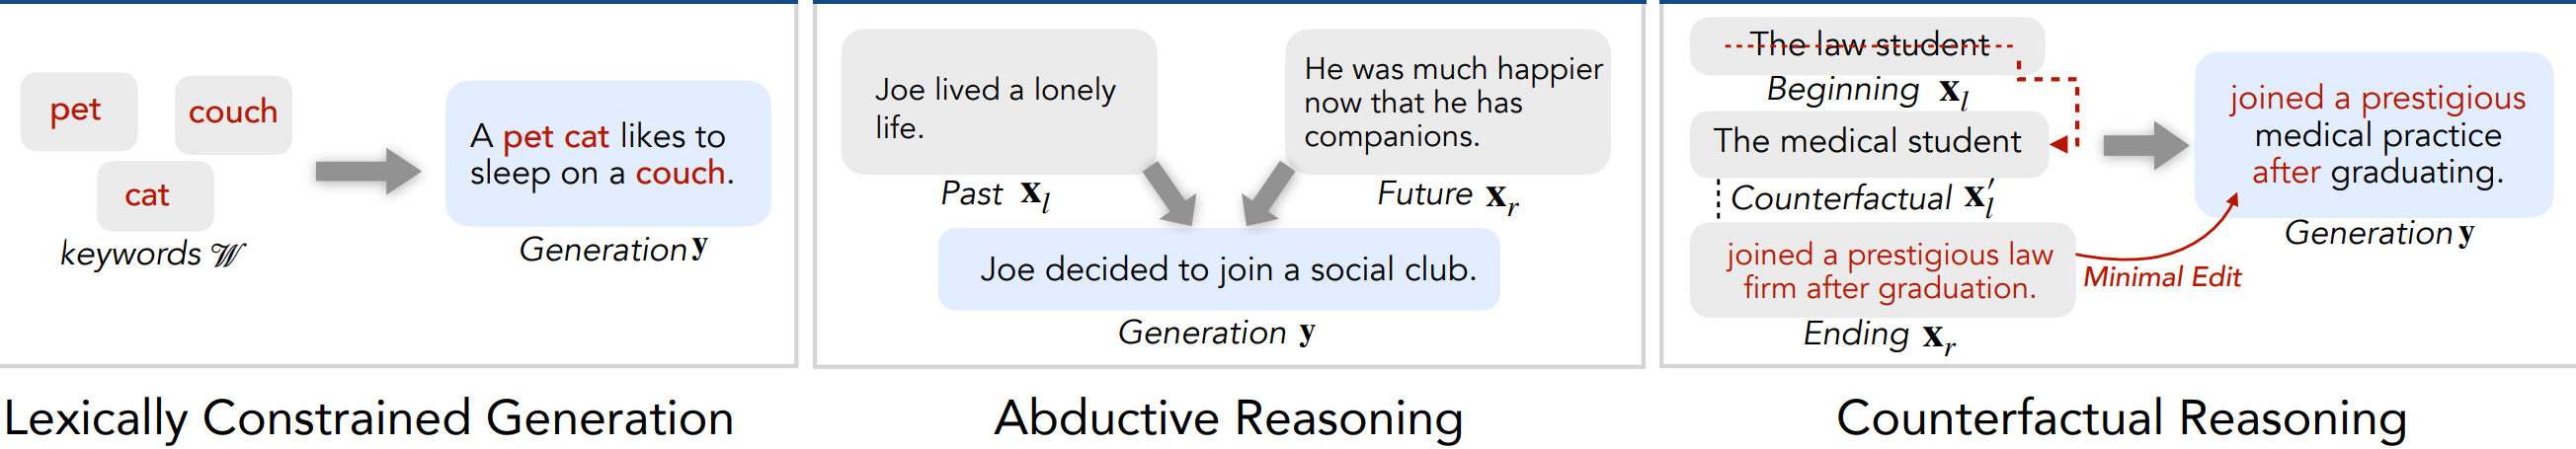
\includegraphics[width=1\textwidth]{fig-1.png}
    % \captionsetup{labelfont=bf,font=footnotesize}
    \caption{Applying CDBD to different constrained generation tasks amounts to specifying an energy function $E$ by plugging in relevant constraint functions. Text in grey boxes is the input, and text in blue boxes is the output.}
    \label{fig:constrained_generation}
\end{figure}

\subsection{Constraints}
\subsubsection{Soft Constraints}
The soft fluency constraint is designed to promote fluency in generated text sequences by leveraging a pre-trained language model. The fluency of a sequence is evaluated based on how closely the generated soft sequence matches the distribution predicted by the language model. The constraint is mathematically represented as:

\begin{equation}
    f_{\overrightarrow{\text{LM}}}(\mathbf{\tilde{y}}) = \sum_{t=1}^{T} \sum_{v \in V} p_{\overrightarrow{\text{LM}}}(v|\mathbf{\tilde{y}}_{<t}) \log \text{softmax} (\mathbf{\tilde{y}}_t(v)),
\end{equation}


where:
\begin{itemize}
    \item \(f_{\overrightarrow{\text{LM}}}(\mathbf{\tilde{y}})\) is the fluency constraint for the soft sequence \(\mathbf{\tilde{y}}\),
    \item \(T\) is the length of the soft sequence,
    \item \(V\) is the vocabulary set,
    \item \(p_{\overrightarrow{\text{LM}}}(v|\mathbf{\tilde{y}}_{<t})\) is the probability of the word \(v\) at position \(t\) predicted by the language model given the preceding soft tokens \(\mathbf{\tilde{y}}_{<t}\),
    \item \(\mathbf{\tilde{y}}_t(v)\) is the logit for word \(v\) at position \(t\) in the soft sequence,
    \item The \(\text{softmax}\) function is applied to \(\mathbf{\tilde{y}}_t(v)\) to convert logits into a probability distribution over the vocabulary for each position \(t\).
\end{itemize}


The inner summation \(\sum_{v \in V}\) computes the negative cross-entropy between the distribution predicted by the language model and the distribution represented by the soft sequence at each position \(t\). The outer summation \(\sum_{t=1}^{T}\) aggregates this measure across the entire sequence, ensuring that the generated sequence is fluent and coherent according to the language model's predictions.

This constraint effectively encourages the generated sequence to be not only fluent but also contextually coherent, making it a powerful tool for generating high-quality, natural-sounding text.

In the context of generating a sequence, \(T\) represents the length of the sequence being generated or evaluated. The knowledge of \(T\) beforehand depends on the specific generation task:

\begin{itemize}
    \item \textbf{Fixed-Length Generation:} For tasks where the desired output length is predetermined, \(T\) is known at the outset. This allows the generation process to be tailored to produce sequences that exactly meet the predefined length.

    \item \textbf{Dynamic Generation:} In scenarios where the sequence ends based on specific criteria (like an end-of-sequence token), \(T\) is not fixed beforehand. Instead, it becomes known only as the generation process unfolds, with the sequence length adapting dynamically based on the content being generated.
\end{itemize}

\subsubsection{Future-token Prediction Constraint}
In applications such as text infilling, the task involves predicting missing tokens within a given sequence, where certain future input tokens remain fixed and are known beforehand. These fixed future tokens should influence the updating of past positions to ensure coherence and contextual relevance throughout the sequence.

For instance, consider the task of updating the missing word in the sentence ``The \_\_ has eight legs.'' It is essential that the predicted word for the blank space not only fits grammatically but also semantically with the future tokens, in this case, ``has eight legs.''

To address this requirement, we introduce a \emph{future-token prediction constraint}. This constraint is designed to adjust the soft tokens in the sequence to maximize the likelihood of the known future input tokens, denoted as \(x_r\). The constraint is mathematically represented as follows:

\begin{equation}
    f_{pred}(\mathbf{\tilde{y}}; \mathbf{x_r}) = \sum_{k=1}^{K} \log {p}_{\overrightarrow{LM}}({x_{r,k}}|\mathbf{\tilde{y}}, {\mathbf{x}_{r,<k}}),
\end{equation}

where:
\begin{itemize}
    \item \(\mathbf{K}\) is the length of the sequence \(\mathbf{x_r}\),
    \item \(p_{\mathbf{\overrightarrow{LM}}}(x_{r,k}|\mathbf{\tilde{y}}, \mathbf{x}_{r,<k})\) represents the probability, predicted by the underlying language model (\(\mathbf{LM}\)), of the future token \(x_{r,k}\) given the soft sequence \(\mathbf{\tilde{y}}\) and all preceding future tokens \(\mathbf{x}_{r,<k}\).
\end{itemize}



In essence, this constraint adjusts the soft sequence \(\tilde{y}\) such that the underlying language model is more likely to predict the future tokens \(x_r\) correctly after being presented with \(\tilde{y}\). This ensures that the generated or updated sequence is not only grammatically correct but also contextually coherent with the fixed future tokens.

\subsubsection{N-gram Similarity Constraint}

In many constrained generation scenarios, requirements are placed on the wording and expression of the generated text sequences. For example, lexically constrained generation tasks require the presence of certain keywords within the text samples, while tasks related to counterfactual reasoning or text editing necessitate that the generated text retains the essence of a reference sequence.

To address these requirements, we introduce an \emph{n-gram similarity constraint}. This constraint is designed to favor sequences that exhibit overlap with a reference sequence \(y^*\) at the n-gram level. The constraint is mathematically expressed as follows:

\begin{equation}
    f_{\text{sim}}(\tilde{\mathbf{y}}; \mathbf{y}^*) = \text{ngram-match}(\tilde{\mathbf{y}}, \mathbf{y}^*),
\end{equation}

where \(\text{ngram-match}(\cdot, \cdot)\) denotes a recent differentiable n-gram matching function, which serves as a differentiable approximation to the BLEU-n metric. This function is capable of quantifying the similarity between the generated sequence \(\tilde{y}\) and the reference sequence \(y^*\) based on their shared n-grams.

When \(n = 1\) and \(y^*\) represents a sequence of keywords, this constraint effectively enforces that \(\tilde{y}\) assigns higher values to the specified keywords (1-grams), ensuring their presence in the generated text. Conversely, when \(n\) is larger and \(y^*\) is a more extensive reference sequence, the constraint encourages \(\tilde{y}\) to resemble \(y^*\) more closely by assigning high values to tokens that constitute n-grams found within \(y^*\).

This n-gram similarity constraint plays a critical role in ensuring that generated text sequences adhere to specified lexical requirements or retain significant elements of reference sequences, thereby enhancing the relevance and coherence of the generated content in accordance with the task-specific constraints.

\subsection{From Soft to Discrete and Fluent Text}

Upon obtaining a soft sequence sample \(\mathbf{\tilde{y}}\) from running Langevin dynamics, our goal is to map this soft sequence to a discrete text sequence. This discrete sequence is considered as the output of COLD decoding. A straightforward approach for this mapping would involve selecting the most-likely token at each position \(t\), defined as \(y_t = \arg\max_v \mathbf{\tilde{y}}_t(v)\). However, this direct method might lead to text that suffers from fluency issues, even when a soft fluency constraint is employed. This is due to the presence of competing constraints that may compromise fluency for satisfying other criteria.

To address these challenges and ensure the fluency of the resulting text, we incorporate the underlying language model (e.g., \( \mathbf{GPT2-XL} \)) as a "guardian" in the process of obtaining the discrete sequence. Specifically, for each position \(t\), the language model is used to produce the top-\(k\) most-likely candidate tokens based on its generation distribution, conditional on the preceding tokens. We denote this set of candidates as \(V_{k_t}\).

From these top-\(k\) candidates, we then select the most likely token according to the soft sample \(\mathbf{\tilde{y}}\):

\begin{equation}
    y_t = \arg\max_{v \in V_{k_t}} \mathbf{\tilde{y}}_t(v).
\end{equation}

This approach is referred to as "top-k filtering." Text generated through this method tends to exhibit higher fluency, as each token is among the top-\(k\) most probable choices according to the language model. Additionally, to facilitate the satisfaction of specific constraints (e.g., n-gram similarity), we may expand the candidate set \(V_{k_t}\) to include tokens that are critical for meeting those constraints, such as in tasks involving abductive reasoning and lexically constrained decoding.

\subsection{Implementation of COLD Decoding}

\subsubsection*{Sample-and-Select}
COLD decoding facilitates the generation of multiple text samples from the distribution induced by the energy function \(E(\mathbf{\tilde{y}})\). Based on the specific requirements of the task, these samples can either be presented as a set of outputs or a single sequence can be selected from the set according to certain criteria (e.g., different energy terms) for tasks as demonstrated in our experiments. This "sample-and-select" approach distinguishes itself from deterministic constrained decoding methods, which focus on optimizing a single sequence, and finds broad application across various generation settings.

\subsubsection*{Initialization}
The soft sequence \(\mathbf{\tilde{y}}\) is initialized using greedy decoding with the language model \(p_{\text{LM}}\) to generate initial output logits. Preliminary experiments indicate that the choice of initialization strategy has a limited impact on the generation results.

\subsubsection*{Noise Schedule}
During each iteration of Langevin dynamics, noise \(\boldsymbol{\epsilon}^{(n)} \sim \mathcal{N}(0, \sigma^{(n)})\) is added to the gradient. We employ a gradually decreasing schedule for \(\sigma^{(n)}\) across iterations, transitioning the decoding process from exploration to optimization. Typically, the noise schedule sets or reduces \(\sigma\) to \(\{1, 0.5, 0.1, 0.05, 0.01\}\) at iterations \(\{0, 50, 500, 1000, 1500\}\), respectively.

\subsubsection*{Long Sequences}
COLD decoding inherently produces a fixed-length sequence \(\mathbf{y} = (y_1, \ldots, y_T)\). To generate longer sequences, particularly in cases where \(y_T\) does not signify the conclusion of a sentence, we utilize \(p_{\text{LM}}\) for a continuation of \(\mathbf{y}\) using greedy decoding.

\subsection{Implementation Details}

The implementation involves initializing parameters and the noise term, setting up the optimizer and scheduler, and executing the optimization loop as follows:

\begin{minted}{python3}
# Initialization
y_logits = init_logits
epsilon = torch.nn.Parameter(torch.zeros_like(y_logits))

# Optimizer and Scheduler Setup
if args.prefix_length > 0:
    optim = torch.optim.Adam([epsilon, prefix_logits], lr=args.stepsize)
else:
    optim = torch.optim.Adam([epsilon], lr=args.stepsize)
scheduler = torch.optim.lr_scheduler.StepLR(optimizer=optim, step_size=args.stepsize_iters,
                                             gamma=args.stepsize_ratio)

# Optimization Loop
optim.zero_grad()
y_logits_ = y_logits + epsilon
# Compute loss in a function (not shown)
if iter < args.num_iters - 1:
    loss.backward()  # Compute gradients
    optim.step()  # Update parameters
    scheduler.step()  # Update learning rate
    last_lr = scheduler.get_last_lr()[0]
\end{minted}


This implementation iteratively updates the parameters to minimize the loss function, incorporating noise to aid in exploring the parameter space. The use of an adaptive learning rate scheduler and the Adam optimizer facilitates efficient and effective optimization.

\subsection{Loss Computation Overview}

The loss computation for models operating in counterfactual, abductive, and lexical modes involves multiple components, including left-to-right (L2R) loss, right-to-left (R2L) loss, and constraint losses. The total loss is a combination of these components, weighted appropriately according to the model configuration.

\subsubsection{Loss Components}

\paragraph{L2R Loss:} The L2R loss is computed using a soft negative log-likelihood function, applied to the model's forward pass logits, after applying a top-k filter and adjusting by an output logits temperature.

\paragraph{R2L Loss:} The R2L loss computation varies based on the mode:
\begin{itemize}
    \item In counterfactual mode, it involves reversing the model's logits, processing them through the backward model, and computing the soft NLL against the adjusted and reversed logits.
    \item In abductive and lexical modes, the logits are flipped, processed through a backward model, adjusted for repetition, and the soft NLL is computed against the filtered and temperature-adjusted logits.
\end{itemize}

\paragraph{Constraint Loss:} Depending on the mode:
\begin{itemize}
    \item Counterfactual mode utilizes a BLEU-like loss computed against a set of n-grams.
    \item Abductive and lexical modes combine a cross-entropy loss and a BLEU-like loss, with the latter weighted by a specific factor.
\end{itemize}

\subsubsection{Total Loss Computation}

The total loss is calculated as a weighted sum of the L2R and R2L losses, alongside the constraint loss, each adjusted by specific weights reflecting the importance of each component and the overall model configuration. The formula for the total loss is:

\begin{multline*}
    \text{loss} = (1.0 - \text{args.constraint\_weight}) \times \text{args.lr\_nll\_portion} \times \text{lr\_nll\_loss} \\
    + \text{args.constraint\_weight} \times (1 - \text{args.lr\_nll\_portion}) \times \text{rl\_nll\_loss} \\
    + \text{args.constraint\_weight} \times \text{c\_loss}
\end{multline*}



This loss is then averaged across the batch for optimization.


\section{Langevin MCMC and Problems in their Implementation}
\subsection{Langevin MCMC}
The core of the Langevin MCMC is the Langevin equation, which is a stochastic differential equation that describes the evolution of a particle in a potential field with some form of friction or resistance, and subject to random fluctuations. In the context of MCMC, the Langevin equation can be discretized to update the chain's state as follows:

\begin{equation}
    x_{t+1} = x_t + \frac{\epsilon^2}{2} \nabla \log p(x_t) + \epsilon Z_t
\end{equation}

where $x_t$ is the state at time $t$, $\epsilon$ is the step size, $\nabla \log p(x_t)$ is the gradient of the log-target distribution at $x_t$, and $Z_t$ is a standard Gaussian random variable. The first term in the update represents a deterministic drift towards higher probability regions, while the second term introduces randomness to explore the state space.

Langevin MCMC is particularly useful in scenarios where the target distribution is known up to a normalization constant, which is common in Bayesian inference problems. It has been successfully applied in various fields such as machine learning, statistical physics, and computational biology, among others.

Langevin MCMC provides an efficient and effective means of sampling from complex, high-dimensional distributions by leveraging gradient information. This leads to faster convergence compared to traditional MCMC methods, making it a valuable tool in the arsenal of statistical and machine learning techniques.

\subsection{Problems in Implementation}
The implementation in question employs the Adam optimizer in an algorithm inspired by Langevin MCMC, as shown in the following equation:

\begin{equation}
    \tilde{\boldsymbol{y}}^{(n+1)} \leftarrow \tilde{\boldsymbol{y}}^{(n)} - \eta \nabla_{\tilde{\boldsymbol{y}}} E(\tilde{\boldsymbol{y}}^{(n)}) + \epsilon^{(n)},
\end{equation}

However, this approach deviates significantly from traditional Langevin MCMC methods. The Adam optimizer's variable learning rates contrast with the constant learning rate required for theoretical consistency in Langevin MCMC, where the standard deviation of the noise term \( \epsilon^{(n)} \) must be proportional to the learning rate \( \eta \).

This critical relationship is absent in their approach, which undermines the fundamental concept of Langevin dynamics—specifically, the proportional scaling of the "temperature" of the sampling with the learning rate. The resulting methodology therefore diverges from Langevin MCMC as it traditionally stands, and does not utilize its mechanism for the purpose of sampling, given that the variance of the noise does not maintain a fixed relationship with the adaptive learning rate. The correct implementation of noise in Langevin MCMC should adhere to the following equation:

\begin{equation}
    \epsilon^{(n)} \sim \mathcal{N}(0, 2\eta),
\end{equation}

The discrepancy between the adaptive learning rates employed by Adam and the requirements of Langevin MCMC suggests that the term 'Langevin' might not be suitably applied in this context. To align with Langevin MCMC, a fixed learning rate should be used, ensuring the noise variance is appropriately scaled and maintains the balance between exploration and exploitation as prescribed by Langevin dynamics.

\section{Proposed Methodology: Barker Proposal MCMC for Sampling}

In this project, we introduce a novel approach to sampling within the MCMC framework, adopting the Barker proposal mechanism. This methodology represents a significant shift from traditional techniques, aiming to improve the exploration of the parameter space through a more nuanced probability-driven update mechanism. The process is delineated as follows:

Firstly, we sample a perturbation vector \(z\) from a Gaussian distribution, \(z \sim \mathcal{N}(0, \sigma^2)\), where \(\sigma^2\) is the variance that dictates the scale of exploration.

Subsequently, we calculate the acceptance probability \(\alpha\) for each proposed move using the Barker formula:
\begin{equation}
    \alpha = \frac{1}{1+e^{-z \cdot \nabla_{y} E(y_k)}},
\end{equation}
where \(y_k\) denotes the current state, \(\nabla_{y} E(y_k)\) is the gradient of the energy function \(E\) at \(y_k\), and \(z\) is the sampled perturbation. This formula ensures a probabilistic balance between exploration and exploitation, modulating the acceptance of new states based on the direction and magnitude of the gradient of the energy function.

The update rule is then applied as follows: With probability \(\alpha\), the next state \(y_{k+1}\) is set to \(y_k + z\), effectively moving in the direction of the perturbation. Conversely, with probability \(1-\alpha\), \(y_{k+1}\) is set to \(y_k - z\), opting for a move against the perturbation. This dual-probability mechanism allows for an adaptive exploration of the space, taking into account both the energy landscape and the stochastic element introduced by \(z\).

\begin{equation}
    y_{k+1} =
    \begin{cases}
        y_k + z & \text{with probability } \alpha   \\
        y_k - z & \text{with probability } 1-\alpha
    \end{cases}
\end{equation}

The Barker proposal MCMC thus introduces a flexible and effective method for sampling, particularly suited for scenarios where navigating complex energy landscapes is essential. By leveraging the gradient of the energy function alongside stochastic perturbations, this approach fosters a more dynamic exploration of the parameter space, potentially enhancing the efficiency and efficacy of the sampling process in diverse applications.

\bibliographystyle{plain} % This will number references in the order they appear in the text
\bibliography{ref} % This is the filename of the .bib file without the extension

\end{document}